\begin{frame}{Structure}
  \tableofcontents
\end{frame}

\section{Neural network ~\newline basics}

\begin{frame}{Neural network}
  \begin{definition}
    (Neural Network)
    A neural network $\Phi$ is a composition of one or multiple layers $\phi$ 
    with compatible input and ouput dimensions:
    \begin{equation*}
      \Phi(x;\Theta) = \phi_{n_L} \lb \phi_{n_L-1} \lb \cdots
      \lb \phi_2(
      \phi_1(x;\theta_1); \theta_2 ) \cdots \rb ; \theta_{n_L-1} \rb ; \theta_{n_L} \rb
    \end{equation*}
    We denote the vector of
    \bemph{all layer parameters} with $\Theta = (\theta_1^T, \dots, \theta_{n_L}^T)^T$.
  \end{definition}
  
  Example: (fully-connected) linear layer
  \begin{equation*}
    \phi(x) = Wx +b
  \end{equation*}
  with parameters $W \in \R^{n_2 \times n_1}$ 
  and $b \in \R^{n_2}$,\\
  i.e. $\theta = (vec(W)^T, b^T)^T \in \R^{n_2 n_1 + n_2}$.
\end{frame}

\begin{frame}{Training data and loss}
  Here: supervised learning

  \begin{block}{Training data}
    $\mathcal{T} = \{(x_1, y_1) \dots, (x_{n_{\text{train}}},y_{n_{\text{train}}}) \}
   \subset \R^{n_x} \times \R^{n_y}$
  \end{block}

  \begin{block}{Mini-batches}
    disjoint subsets $\mathcal{B}_1, \dots, \mathcal{B}_{n_{\text{b}}}$
    with $\mathcal{T} = \mathcal{B}_1 \cup \cdots \cup \mathcal{B}_{n_{\text{b}}}$
  \end{block}

  \begin{block}{Loss}
    \begin{equation*}
      L(\mathcal{B}; \Theta) = \sum_{(x_i,y_i) \in \mathcal{B}} l(\Phi(x_i; \Theta), y_i),
    \end{equation*}
    where $l : \R^{n_y} \times \R^{n_y} \to \R$ gives the loss for an 
    individual training sample.
  \end{block} 
\end{frame}

\begin{frame}{Gradient descent}
  learning rate $\gamma \in  \R$

  epoch $i \in \N$
  \begin{block}{Gradient descent}
    \begin{equation*}
      \Theta_{i+1} = \Theta_i - \gamma \grad[\Theta]{L(\mathcal{T};\Theta_{i})}
    \end{equation*}
  \end{block}

  If the training data is split into mini-batches:
  \begin{block}{Stochastic Gradient descent}
    \begin{equation*}
      \Theta_{i+1} = \Theta_i - \gamma \grad[\Theta]{L(
        \mathcal{B}_{((i \textrm{ mod } n_{\text{b}}) + 1)};
        \Theta_{i})}
    \end{equation*}
  \end{block}

  different gradient descent flavors, for example Adam, ...
\end{frame}

\section{Hamiltonian Systems}

\begin{frame}{Hamiltonian system}
  \begin{equation*}
    J := \begin{pmatrix}
      0 & I_d \\
      -I_d & 0
    \end{pmatrix}, \,
    d \in \N
  \end{equation*}

  \begin{definition}
    A \bemph{Hamiltonian (ODE) system} can be written in canonical form as
    \begin{align*}
      \dot{y}(t) &= J \grad{H}(y(t)) \quad \text{for } t \in I \subset \mathbb{R} \\
      y(t_0) &= y_0
      ,
    \end{align*}
    where $y: I \subset \mathbb{R} \to \mathbb{R}^{2d},\, t \mapsto y(t) = (q(t),p(t))$ and 
    $y_0 = (q_0, p_0) \in \mathbb{R}^{2d}$ the initial value at $t_0 \in I$.
    The function $H: \mathbb{R}^{2d} \to \mathbb{R}$ is called the \bemph{Hamiltonian}
    or the \bemph{total energy}. The entries of $q = q(t) \in \mathbb{R}^d$ are called 
    \bemph{generalized coordinates}
    and the entries of $p=p(t) \in \mathbb{R}^d$ are called \bemph{conjugate momenta}. 
    The \bemph{phase space} $\mathcal{V} = \mathbb{R}^{2d}$ has even dimension for Hamiltonian systems.
  \end{definition}
\end{frame}

\begin{frame}[c]{Conservation of the total energy}
  \centering
  \begin{equation*}
    \ddt H(y(t)) = \lsb \grad{H}(y(t)) \rsb^T \dot{y}(t) = 
    \lsb \grad{H}(y(t)) \rsb^T J \grad{H}(y(t)) = 0
  \end{equation*}
\end{frame}

\begin{frame}{Flow}
  flow of a Hamiltonian system
  \begin{equation*}
    \phi_{t,H}\begin{pmatrix}
      q_0 \\
      p_0
    \end{pmatrix}
    = \begin{pmatrix}
      q(t; q_0, p_0) \\
      p(t; q_0, p_0)
    \end{pmatrix}
  \end{equation*}

  \begin{definition}
    A differentiable map $\phi : U \to \mathbb{R}^{2d}$ (where $U \subset \mathbb{R}^{2d}$ is an open set)
    is called symplectic if the Jacobian matrix $\jac{\phi}{x}$ is symplectic everywhere, i.e.
    \begin{equation*}
      \lb \jac{\phi}{x} \rb^T J \lb \jac{\phi}{x} \rb = J
      .
    \end{equation*}
  \end{definition}

  \bemph{The flow $\phi_{t,H}$ of a Hamiltonian system is symplectic!} (Poincaré 1899)
\end{frame}

\section{SympNets: ~\newline Symplectic networks}

\begin{frame}[c]{Block operator}
  For $q,p \in \R^{d}$ and maps $f_{11}, f_{12}, f_{21}, f_{22} : \R^d \to \R^d$,
  we define the block operator as
  \begin{equation*}
    \begin{bmatrix}
      f_{11} & f_{12} \\
      f_{21} & f_{22}
    \end{bmatrix}
    \qpvec
    := \begin{pmatrix}
      f_{11}(q) + f_{12}(p) \\
      f_{21}(q) + f_{22}(p)
    \end{pmatrix} \in \R^{2d}
    .
  \end{equation*}
\end{frame}

\begin{frame}{The building block}
  \begin{definition}
    (Unit Triangular Layer) A layer $\phi : \mathbb{R}^{2d} \to \mathbb{R}^{2d}$ 
    is called a unit triangular layer with \bemph{layer transform}
    \begin{equation*}
      \layertf : \mathbb{R}^d \to \mathbb{R}^d,\, p \mapsto \layertf(p)
    \end{equation*}
    and bias parameter $b \in \R^{2d}$, if $\phi$ can be expressed as
    \begin{equation*}
      \phi_\up \qpvec = \uppersympop{\layertf} + b
      = \begin{pmatrix}
        q + \layertf(p) \\
        p
      \end{pmatrix} + b \quad \text{(upper unit triangular layer)}
    \end{equation*}
    or
    \begin{equation*}
      \phi_\low \qpvec = \lowersympop{\layertf} + b
      = \begin{pmatrix}
        q \\
        \layertf(q) + p
      \end{pmatrix} + b. \quad \text{(lower unit triangular layer)}
    \end{equation*}
  \end{definition}

  \bemph{A unit triangular layer is symplectic iff. the Jacobian of the 
  layer transfrom $\layertf$ is symmetric everywhere.}
\end{frame}

\begin{frame}[c]{Linear layers}
  The \bemph{linear layers} are given by the layer transform
  \begin{equation*}
    \layertf(p) = Sp
  \end{equation*}
  with a symmetric matrix $S \in \R^{d \times d}$ parametrized\\
  by $A \in \R^{d \times d}$ via $S=A^T+A$.
  \vspace{1cm}

  A linear layer can be expressed with matrix-vector multiplication:
  \begin{equation*}
    \phi_\up \qpvec = \begin{pmatrix}
      I & S \\
      0 & I
    \end{pmatrix} \qpvec + b
    .
  \end{equation*}
\end{frame}

\begin{frame}[c]{Activation layers}
  The \bemph{activation layers} are given by the layer transform
  \begin{equation*}
    \layertf(p) = \lb a_i \activation(p_i) \rb_{i=1}^d
  \end{equation*}

  with:
  \begin{itemize}
    \item an activation function $\activation$
    \item coefficients $a \in \R^d$ 
  \end{itemize}
\end{frame}

\begin{frame}[c]{Gradient layers}
  The \bemph{gradient layers} are given by the layer transform
  \begin{equation*}
    \layertf(p) = K^T \bigg( a_j \activation \lb (Kp)_j + c_j \rb \bigg)_{j=1}^n
  \end{equation*}

  with:
  \begin{itemize}
    \item an activation function $\activation$
    \item width $n \in \N$ ($n \gg d$)
    \item parameters $a,c \in \R^n$ and $K \in \R^{n \times d}$
  \end{itemize}
\end{frame}

\section{Convolution for ~\newline SympNets}

\begin{frame}[c]{Convolution vs. Cross-correlation}
  Given two discrete functions $f,g \in \mathbb{R}^\mathbb{Z}$, 
  \bemph{convolution} is defined as 
  \begin{equation*}
    *: \mathbb{R}^{\mathbb{Z}} \times \mathbb{R}^{\mathbb{Z}} \to \mathbb{R}^{\mathbb{Z}},
    \quad (f*g)(\tau) = \sum^{\infty}_{a=-\infty} f(a) g(\tau - a)
    .
  \end{equation*}

  \bemph{Cross-correlation} is defined as
  \begin{equation*}
    \star: \mathbb{R}^{\mathbb{Z}} \times \mathbb{R}^{\mathbb{Z}} \to \mathbb{R}^{\mathbb{Z}},
    \quad (f \star g)(\tau) = \sum^{\infty}_{a=-\infty} f(a) g(\tau + a)
    .
  \end{equation*}
\end{frame}

\begin{frame}[c]{Valid cross-correlation}
  \begin{definition}[Valid cross-correlation]
    We define the valid cross-correlation of a finite-dimensional kernel $k \in \mathbb{R}^{n_k}$ and 
    a finite-dimensional input $x \in \mathbb{R}^{n_x}$ with $n_x \geq n_k$ as
    \begin{equation*}
      \star_{\text{v}} : \mathbb{R}^{n_k} \times \mathbb{R}^{n_x} \to \mathbb{R}^{n_x-n_k+1},
      \quad \star_{\text{v}}(k,x) := \mathcal{I}_{n_x-n_k+1}^{\text{inv}} (
        \mathcal{S}_{-1}( \mathcal{I}_{n_k}(k)) \star \mathcal{I}_{n_x}(x)
      )
      .
    \end{equation*}
  \end{definition}

  Example:
  $k \in \R^3$,
  $x \in \R^6$,
  $y := \star_{\text{v}}(k,x) \in \R^4$

  \vspace{0.3cm}
  \centering
  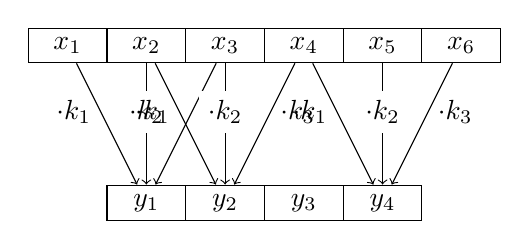
\begin{tikzpicture}
    \foreach \i in {1,2,3,4,5,6} {
      \node (x\i) [draw, minimum width=1cm] at (\i-1, 0) {$x_\i$};
    }
    \foreach \i in {1,2,3,4} {
      \node (y\i) [draw, minimum width=1cm] at (\i, -2) {$y_\i$};
    }

    \onslide<1> {
      \draw [->] (x1) edge node[left,pos=0.4]{$\cdot k_1$} (y1) ;
      \draw [->] (x2) edge node[fill=white,pos=0.4]{$\cdot k_2$} (y1);
      \draw [->] (x3) edge node[right,pos=0.4]{$\cdot k_3$} (y1);
    }

    \onslide<2> {
      \draw [->] (x2) edge node[left,pos=0.4]{$\cdot k_1$} (y2) ;
      \draw [->] (x3) edge node[fill=white,pos=0.4]{$\cdot k_2$} (y2);
      \draw [->] (x4) edge node[right,pos=0.4]{$\cdot k_3$} (y2);
    }

    \onslide<3> {
      \draw [->] (x4) edge node[left,pos=0.4]{$\cdot k_1$} (y4) ;
      \draw [->] (x5) edge node[fill=white,pos=0.4]{$\cdot k_2$} (y4);
      \draw [->] (x6) edge node[right,pos=0.4]{$\cdot k_3$} (y4);
    }
  \end{tikzpicture}
\end{frame}

\begin{frame}{Padding}
  \begin{definition}[Constant padding]
    Given the padding values $l,r \in \mathbb{R}^m$, we define constant padding 
    $c_{\text{pad},m}$ as
    \begin{equation*}
      c_{\text{pad},m} : \mathbb{R}^d \to \mathbb{R}^{d+2m},
      \quad c_{\text{pad},m}(x) = c_{\text{pad},m}(x;l,r) := \lb l^T, x^T, r^T \rb^T
      .
    \end{equation*}
  \end{definition}

  \vspace{0.3cm}
  Example:
  $l,r \in \R^3$,
  $x \in \R^6$

  \vspace{0.3cm}
  \centering
  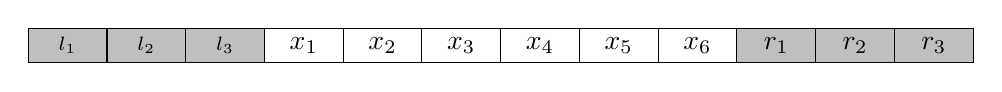
\begin{tikzpicture}
    \node [draw, minimum width=1cm,fill=lightgray] at (0, 0) {\scriptsize$l_1$};
    \node [draw, minimum width=1cm,fill=lightgray] at (1, 0) {\scriptsize$l_2$};
    \node [draw, minimum width=1cm,fill=lightgray] at (2, 0) {\scriptsize$l_3$};
    \foreach \i in {1,2,3,4,5,6} {
      \node [draw, minimum width=1cm] at (\i+2, 0) {$x_\i$};
    }
    \node [draw, minimum width=1cm,fill=lightgray] at (9, 0) {$r_1$};
    \node [draw, minimum width=1cm,fill=lightgray] at (10, 0) {$r_2$};
    \node [draw, minimum width=1cm,fill=lightgray] at (11, 0) {$r_3$};
  \end{tikzpicture}
\end{frame}

\begin{frame}{Padding}
  \begin{definition}[Symmetric padding]
    We define symmetric padding as
    \begin{equation*}
      s_{\text{pad},m} : \mathbb{R}^d \to \mathbb{R}^{d+2m},
      \quad s_{\text{pad},m}(x) := (
        \underbrace{x_m, x_{m-1} \dots, x_1}_{m \text{ values}}, \,
        \underbrace{x_1, x_2 \dots, x_d}_{d \text{ values}}, \,
        \underbrace{x_d, x_{d-1} \dots, x_{d-m+1}}_{m \text{ values}}
      )^T
      .
    \end{equation*}
  \end{definition}

  \vspace{0.3cm}
  Example:
  $x \in \R^6$

  \vspace{0.3cm}
  \centering
  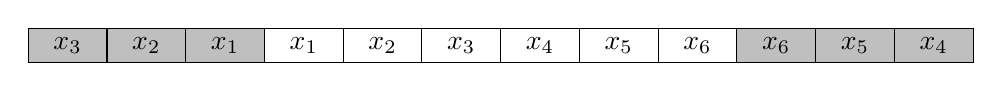
\begin{tikzpicture}
    \node [draw, minimum width=1cm,fill=lightgray] at (0, 0) {$x_3$};
    \node [draw, minimum width=1cm,fill=lightgray] at (1, 0) {$x_2$};
    \node [draw, minimum width=1cm,fill=lightgray] at (2, 0) {$x_1$};
    \foreach \i in {1,2,3,4,5,6} {
      \node [draw, minimum width=1cm] at (\i+2, 0) {$x_\i$};
    }
    \node [draw, minimum width=1cm,fill=lightgray] at (9, 0) {$x_6$};
    \node [draw, minimum width=1cm,fill=lightgray] at (10, 0) {$x_5$};
    \node [draw, minimum width=1cm,fill=lightgray] at (11, 0) {$x_4$};
  \end{tikzpicture}
\end{frame}

\begin{frame}{Convolution layers}
  
\end{frame}

\section{Normalization for ~\newline SympNets}

\begin{frame}{Overview}
  \todo{TODO add table of all layer transforms?}
\end{frame}

\section{Numerical experiments}